\documentclass[12pt]{article}
\usepackage{graphicx,amsmath}
\usepackage{epsfig}

\topmargin=-.5in \oddsidemargin=0in \textwidth=6.5in
\textheight=9in

\parindent 0.0in
\parskip .20in

\def\balpha{\pmb{\alpha}}
\def\bbeta{\pmb{\beta}}
\def\bgamma{\pmb{\gamma}}
\def\bdelta{\pmb{\delta}}
\def\bmu{\pmb{\mu}}
\def\bsigma{\pmb{\sigma}}
\def\bphi{\pmb{\phi}}
\def\bTheta{\pmb{\Theta}}
\def\btheta{\pmb{\theta}}
\def\btau{\pmb{\tau}}
\def\bomega{\pmb{\omega}}

\def\bX{\pmb{X}}
\def\bY{\pmb{Y}}
\def\bZ{\pmb{Z}}
\def\bJ{\pmb{J}}
\def\bV{\pmb{V}}
\def\bR{\pmb{R}}
\def\bW{\pmb{W}}


%\psdraft

\begin{document}
\begin{center}
{\Large Hierarchical Bayes models for daily rainfall time series at multiple locations from different data sources}
\vspace{1in}\\
By Kenneth E. Shirley
\end{center}



\newpage

\section{Motivation}

Crop yields respond to rainfall and temperature, but averaged decadal or even average monthly rainfall can obscure the affects of weather on yields. Frequent exposure to extreme temperatures (high and lows) matters tremendously (Schlenker 2009). Furthermore, the daily variation in other variables, such as soil moisture have been found to be equally important, and if not accounted for, allow for temperature's effect to be overstated (Ortiz 2014). Specifically, the NUMBER of times and WHEN a crop is exposed to highs/lows in temperature and moisture is crucial, which decadal or monthly measures cannot capture. [Is this disingenuous if we don't have temperature but just rainfall amount?]

Daily statistics and extremes of weather often have a greater impact on end-users than climatological averages. For example, although seasonal rainfall totals and average temperatures can provide a general guide to crop yields, plants are also extremely sensitive to extreme weather events over a few hours (Schlenker, 2009, Ortiz 2014), especially during flowering or pod-set.  A classic example is in groundnut, where high temperatures during the one or two days of flowering leads to pod death and plant death (Wheeler et al, 1996; Wheeler et al, 2000), or in maize, where a dry spell over the short Anthesis Tasselling Interval has a well measured and catastrophic impact on yields (Bola�os and Edmeades (1996)).  Similar impacts can be seen in hydrology, where extreme rainfall events that are often of more interest to flood modellers than seasonal averages (REFERENCE), or in climate science, where it is crucial to be able to convert projections of regional averages into changes in local weather (REFERENCE).    

The ability to generate realistic daily time-series of weather is therefore valued in many end-user applications such as hydrological, climate or crop simulation modelling, especially over regions of the world where there are sparse ground based weather station networks.  The technique for producing such time series has moved from deterministic weather models where rainfall follows a stochastic markov process where transition probabilities dictate the chance of rain, give only the particular state. As in (weather generation game) the seminal papers in this area are xxxx. The paper also reviews the techniques of XXX and YYYY[HELEN]. The objective in any of these approaches is to be able to simulate long synthetic time-series of weather that reflect key observed statistics in the region of interest e.g. means, dry spell lengths, or probability of extreme events occurring.  

The Hierarchal Bayes method goes beyond the markov approach for several reasons: 
[ assumes simplistic relationships between weather variables, and regional climate modelling is still in its infancy over many regions, with well documented problems in modelling variables such as rainfall.  But you guys can incorporate all the information you have, so multiple time-series at a location, SSTs etc without knowing the exact prior relationship]

Recently, there has been a high level of interest in spatially correlated weather generators, which would have a clear benefit when considering modelling river basins or regional food security.  Incorporating spatial correlation is also key when one considers that most weather events such as droughts or floods have a high impact precisely because they are spatially correlated, regional events, thus incorporating observed spatial correlations into a well calibrated stochastic approach is likely to lead to more realistic impact models.  Several different techniques and methods have been suggested.  The MarkSim weather generator uses spatially correlated input grids of statistics to allow one to allow estimation at a site where there are no observations (Jones and Thornton, 1993). Wilks (1999,1998) extended a richardson weather generator by driving it with a grid of spatially correlated random numbers.  More recently this approach was extended in the GIST weather generator, incorporates spatial correlation through the use of correlation matrices to sample from a cumulative probability function at each location (Baigorria and Jones, 2010), while Kleiber et al (2012) suggests the use of latent Gaussian processes.  In 2012. Greatrex (2012) proposed a geostatistical sequential simulation approach coupled to a markov generator, which would allow spatially correlated ensembles of maps of rainfall to be generated.  It is important to note that many of these approaches rely on a large amount of observed and calibrated data, for example a dense station network to create variograms [EXPLAIN].   

Then move onto the heirarchical bayes approach and discuss the sanso guenni and related papers......
#http://iri.columbia.edu/climate/forecast/tutorial2/

The hierchacal bayesian estimation is a modeling approach first employed in XXXXX (KENNY?). The approach has two steps or levels: the parameters describing the effect of say satellite information in describing rainfall, and then given those parameters, the probability that rainfall actually occurred. We also assume that given the parameters, the probability of rainfall follows a particular model such as a probit. Use initial crude estimates of betas, an interative process called Gibbs sampling is used to estimate the parameter conditional on the current estimates of the other parameters by making a random draw from the conditional distribution. After a burn in period, the estimates from several different "chains" converge to the correct estimates for each parameter. 

The approach has been broadened to incorporate features such as 
non-stationarity sanso
kleiber

The novelty of our approach is our ability to account for two levels of the rainfall time series information at each site: 1) both the location of the measurement and 2) the instrument used to measure, as well to incorporate. In addition, we 3) estimate the the spatial covariance between all these series and 4) the noise or error in recording rainfall due to the instrument itself. By incorporating several layers of information sources for each site in which we would like to predict weather, we are adding more information to the parameter estimates and, hopefully, improving out-sample predictions. Because we used daily data to fit our model, our simulated data and out-of-sample predictions are daily, which allows us to compute statistics sensitive to daily measurements: probability of rainfall, dry spells, and extreme rainfall. 

The remainder the paper is as follows. In Section 



\section{Procedure}
We model a set of 15 time series of daily rainfall in Ethiopia during the time period from 1992 to 2010, where these 15 time series come from six different locations, and each location has at least two time series of daily rainfall associated with it. The reason we observed multiple time series for each location is that for each location we have multiple sources of data, including rain station data and satellite-based rainfall proxy data. The statistical challenge to modeling such data is to separately estimate the spatial variability between locations and the within-location measurement-based variability. A standard hierarchical model with sets of 15 exchangeable parameters -- one for each time series -- would conflate these two sources of variation. The model we introduce here -- a hierarchical Bayesian model with one level for locations, and another level for multiple data sources within a location -- explicitly models each of these two sources of variation.

Figure~\ref{fig_ethiopia_map} shows the six locations from which the daily rainfall time series are measured. The names of the locations are Hagere Selam, Maykental, Mekele, Abi Adi, Agibe, and Adi Ha. The last of these, Adi Ha, is the location we are most interested in, because we wish to provide rainfall insurance for farmers who live there. Specifically, we want to model rainfall at one of the automated rain stations at Adi Ha, which is one of the 15 time series in our data set, but is also the series that has the least amount of observed data -- only about 200 days worth of data from 2009.

\begin{figure}[htbp]
\begin{center}
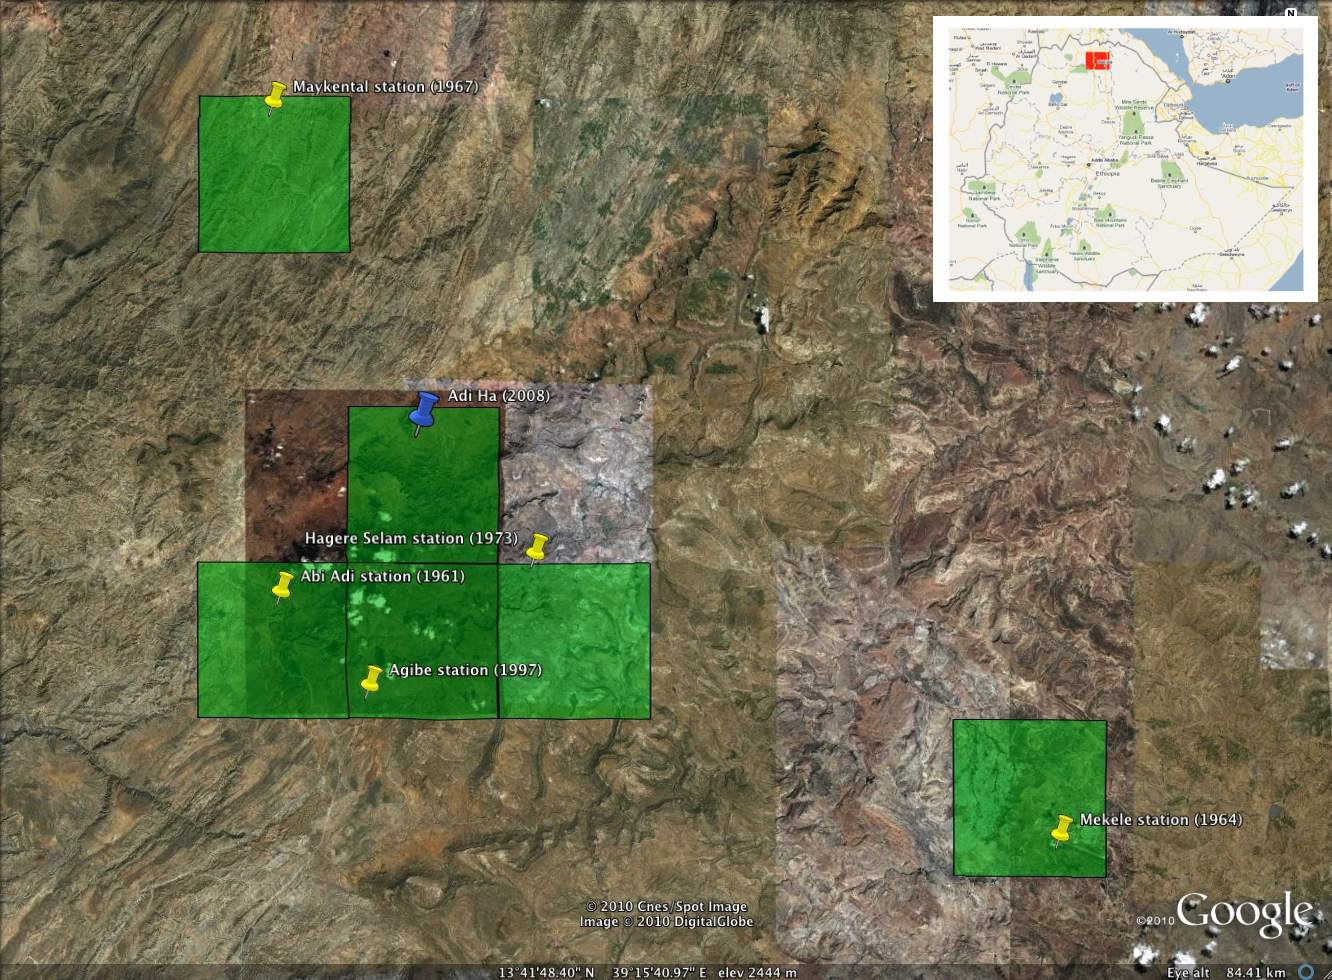
\includegraphics[width=4.5in]{fig_ethiopia_papermap.jpg}
\caption{A map of the 6 locations, where the green squares denote ARC pixels and the pins denote rain station locations. The inset in the upper right corner shows the area of the map with a red rectangular box; this region is in north central Ethiopia.}
\label{fig_ethiopia_map}
\end{center}
\end{figure}

The specifics of the data are as follows:
\begin{itemize}
\item For the first five locations, we have rain station data as well daily measurements from a satellite product called ARC, which is a rainfall proxy based on the temperature of the clouds over an area of about one hundred square kilometers. This comprises $ 5 \times 2 = 10$ time series.
\item For the sixth location, Adi Ha, we have five separate data sources:
\begin{enumerate}
\item One reliable rain station from which we only have 200 days of data from 2009-2010; this is the time series in which we have the most interest, because it is a new, accurate rain station on which we want to base insurance contracts.
\item One unreliable rain station from which we have about 7 years of data from 2000-2009, with about 2 years of missing data interspersed.
\item The ARC satellite proxy.
\item Two additional satellite proxies that are different from ARC.
\end{enumerate}
\end{itemize}

Figure~\ref{fig_overlap} shows the range of observed and missing data for each of these 15 time series; note that the time scale goes back to 1961 for one of the rain stations, but for simplicity, we only consider the time span of 1992-2010 in our model fit, because this span contains most of the data.

\begin{figure}[htbp]
\begin{center}
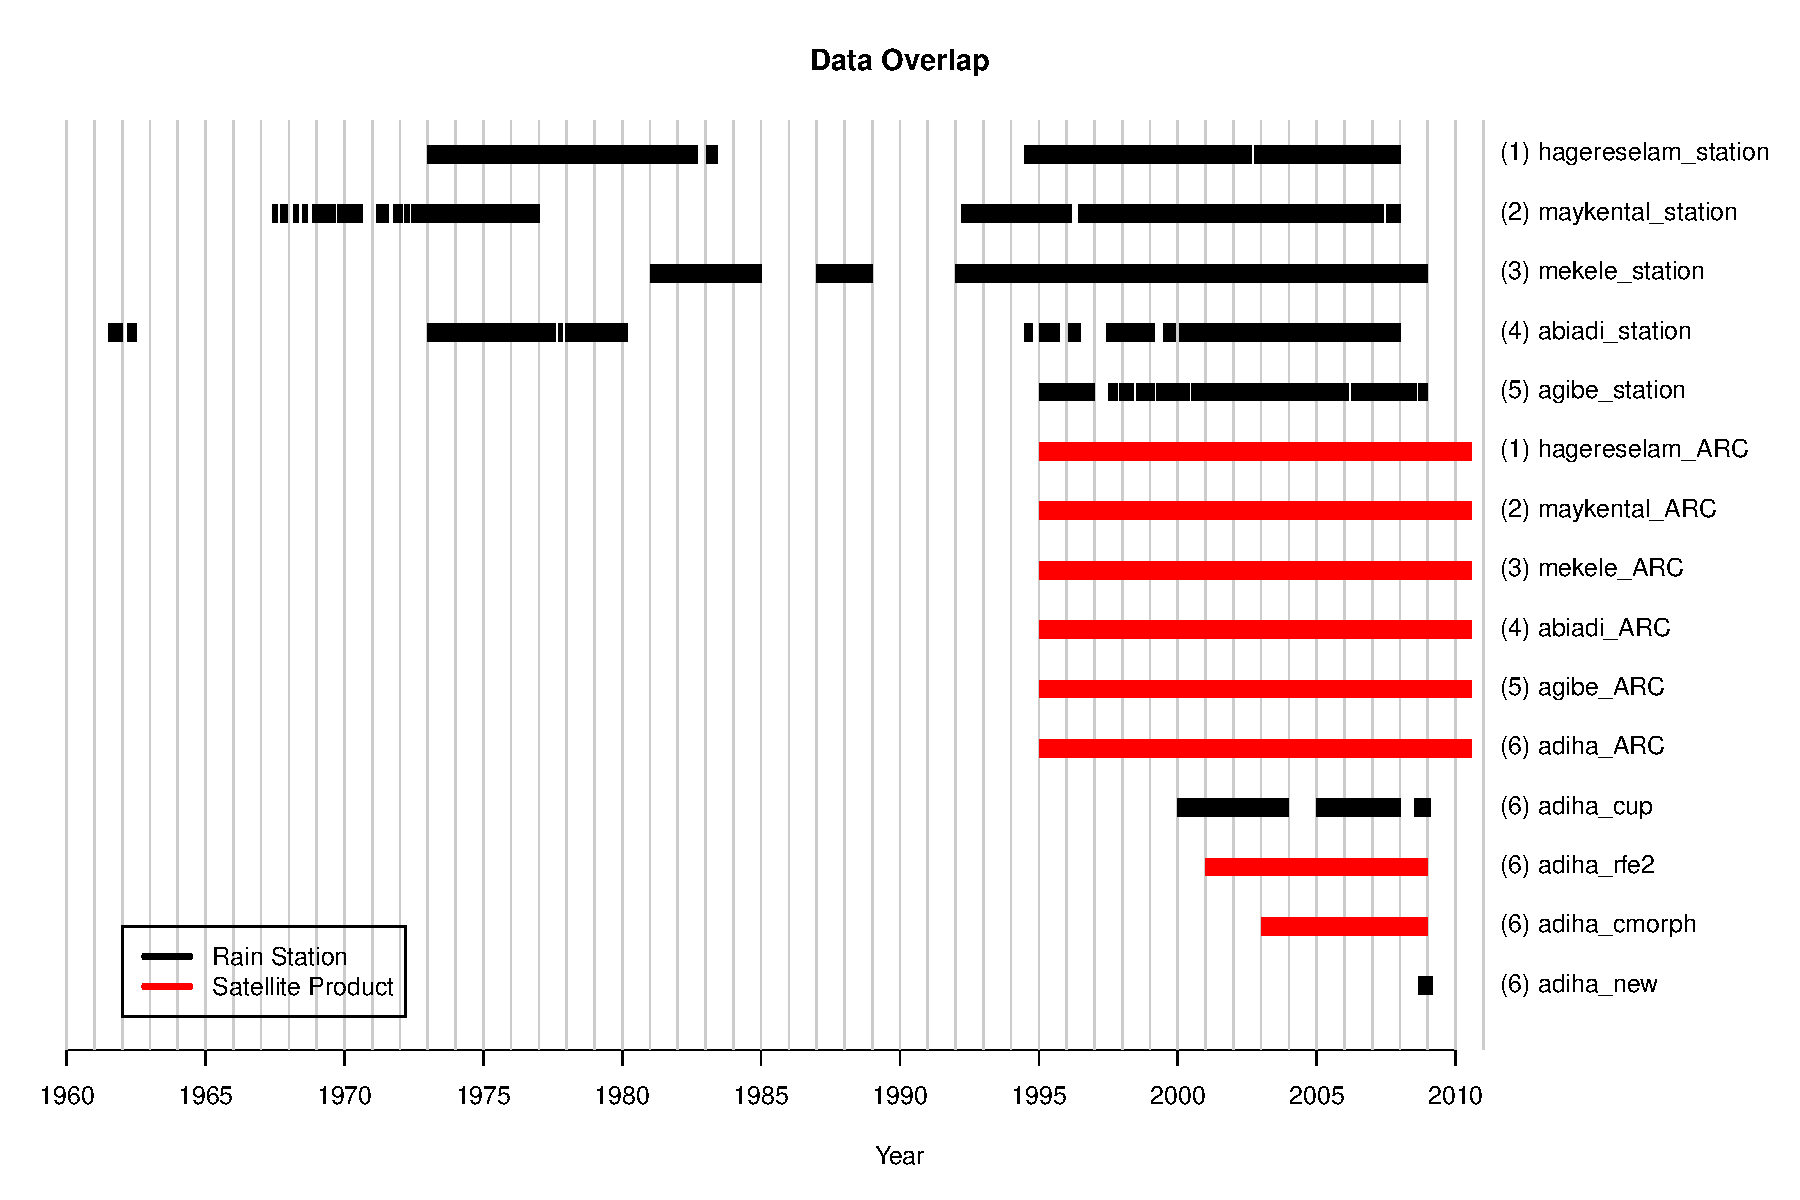
\includegraphics[width=5.0in]{fig_observed_data_new.pdf}
\caption{A visualization of the observed data for each of the 15 time series we model. The black hash marks denote rain station data, and the red hash marks denote satellite-based data.}
\label{fig_overlap}
\end{center}
\end{figure}

Table~\ref{tab_summary} contains some background information and summary statistics related to each time series of daily rainfall. For each time series we record the latitude, longitude, and elevation of the location where measurements were made, and the number of days of observed data. The maximum distance between locations is about 70 kilometers (between Mekele in the southeast and Maykental in the northwest).
\begin{table}[htdp]
\caption{Background information about the 15 time series}
\begin{center}
\begin{tabular}{|l|l|l|l|r|r|}
\hline
 & Site & Latitude & Longitude & Elev. (m) & Num. Obs \\
\hline
1 & Hagere Salaam & $13^\circ$ 38' 49'' & $39^\circ$ 10' 19'' & 2625 & 4887 \\
2 & Hagere Salaam (ARC) & '' & '' & '' & 5632 \\
3 & Maykental & $13^\circ$ 56' 13'' & $38^\circ$ 59' 49'' & 1819 & 5620 \\
4 & Maykental (ARC) & '' & '' & '' & 5632 \\
5 & Mekele & $13^\circ$ 28' 1'' & $39^\circ$ 31' 1'' & 2247 & 6205 \\
6 & Mekele (ARC) & '' & '' & '' & 5632 \\
7 & Abi Adi & $13^\circ$ 37' 19'' & $39^\circ$ 0' 10'' & 1849 & 4205 \\
8 & Abi Adi (ARC) & '' & '' & '' & 5632 \\
9 & Agibe & $13^\circ$ 33' 43'' & $39^\circ$ 3' 43'' & 1952 & 4722 \\
10 & Agibe (ARC) & '' & '' & '' & 5632 \\
11 & Adi Ha (ARC) & $13^\circ$ 43' 48'' & $39^\circ$ 05' 38'' & 1713 & 5632 \\
12 & Adi Ha (Rain Station - Manual) & '' & '' & '' & 2769 \\
13 & Adi Ha (RFE2) & '' & '' & '' & 2920 \\
14 & Adi Ha (CMorph) & '' & '' & '' & 2190 \\
15 & Adi Ha (Rain Station - Automatic) & '' & '' & '' & 186 \\
\hline
\end{tabular}
\end{center}
\label{tab_summary}
\end{table}%

\section{Exploratory Data Analysis}
In this part of Ethiopia, the rainy season lasts roughly from June to October. Figure~\ref{fig_eda} shows the percentage of rainy days and the average amount of rain as a function of the time of year for each time series. The basic modeling strategy will be to use a set of periodic functions to model rainfall as a function of the season of the year.
\begin{figure}[ht]
\begin{center}
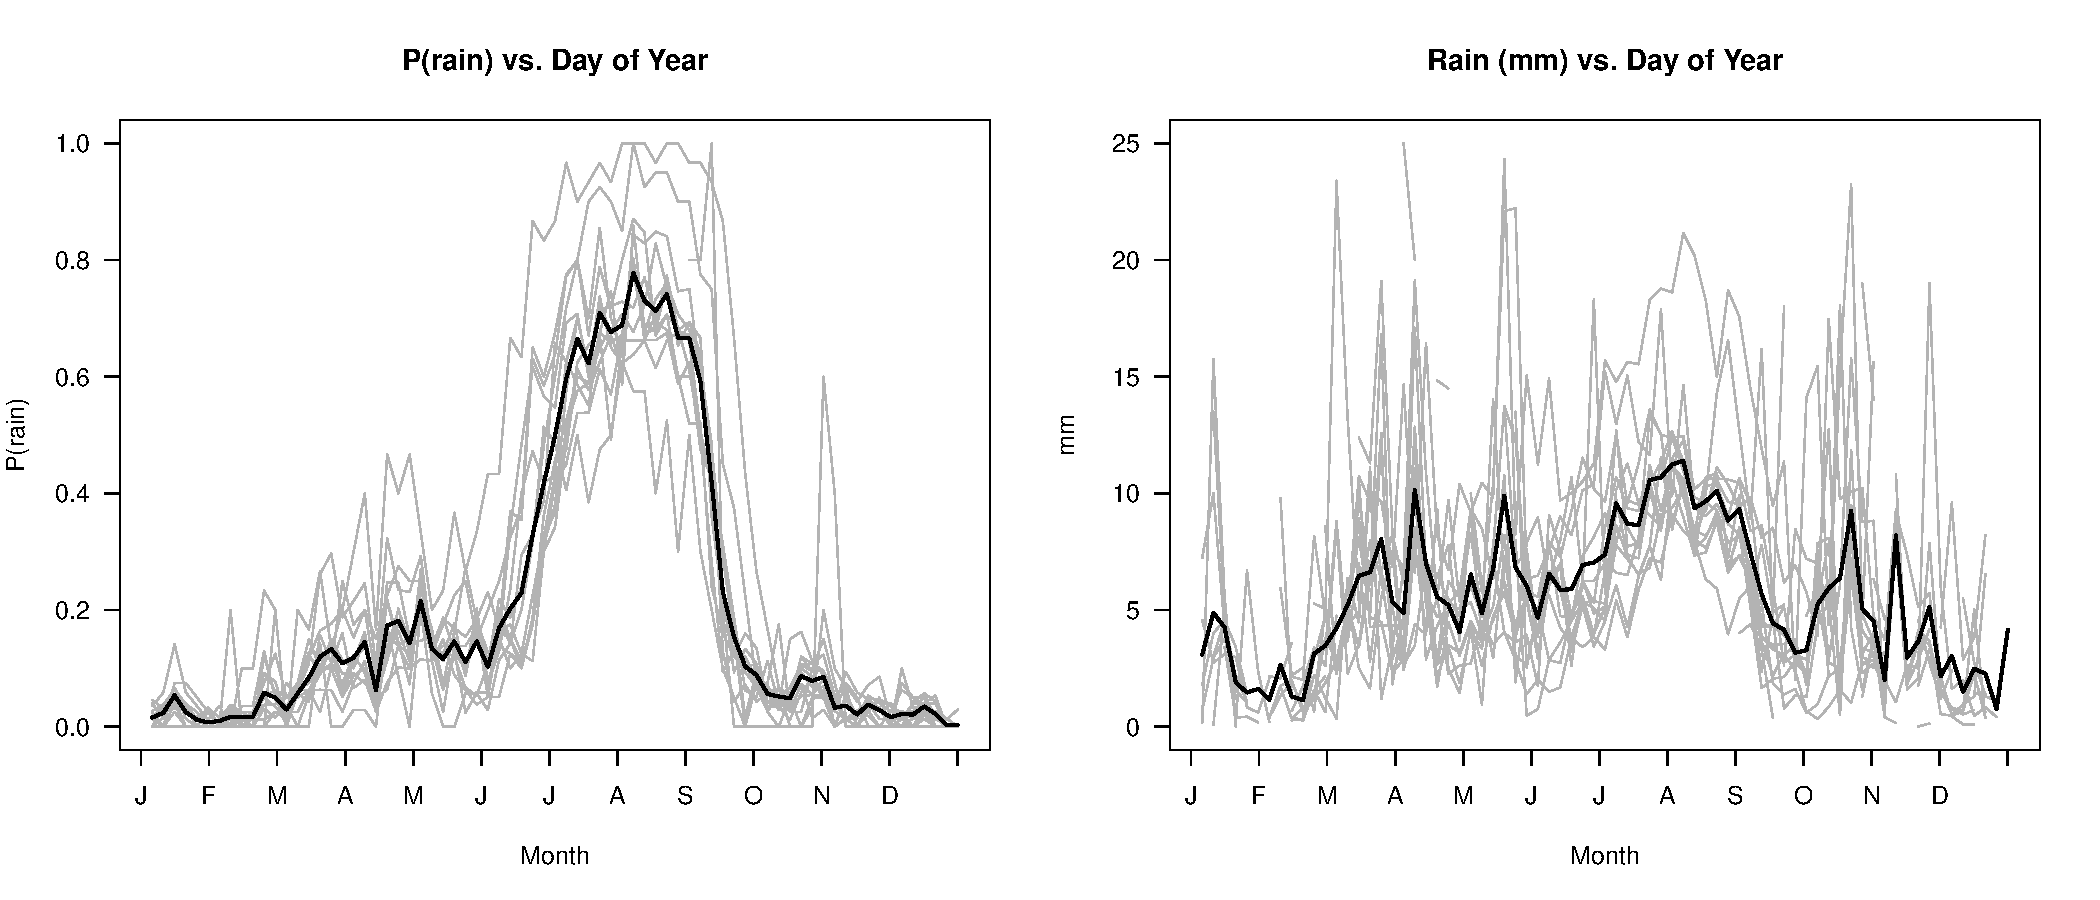
\includegraphics[width=6.5in]{fig_eda.pdf}
\caption{Plots of the percentage of rainy days (pooled into 5-day bins) and the average amount of rain as a function of the season. The gray lines are for each of the 15 individual time series, and the black lines are averaged across all 15 time series.}
\label{fig_eda}
\end{center}
\end{figure}

We are also interested in the difference, on average, between the measurements of rainfall based on the ARC satellite proxy and the rain stations. Comparing rainfall frequencies pooled over 5-day periods, averaging across all parts of the year and all five locations with exactly one rain station and one ARC measurement, we find that the ARC records about 3\% fewer days of rainfall than the rain stations. Across locations, this difference ranges from about -6\% (Hager Selam) to  +1\% (Agibe).



\section{The Model}
Our model consists of two main components: a model for the binary variable of whether or not it rains on a given day (called the frequency model), and a model for the amount of rainfall, given that there was rainfall (called the intensity model). In this paper, we are most interested in the frequency model; the methods we use to model frequency, though, could also be used to model intensity.

Let us first set up some notation. Let $S=6$ denote the number of locations where we measure rainfall, and $\bJ = \{2,2,2,2,2,5\}$ is the vector denoting the number of daily rainfall time series observed for each of the $S$ locations. The total number of days in our time series is $T=6679$ days, from 1/1/1992 through 7/28/2010. Let $V_{stj}$ denote the amount of rainfall, measured in mm, for location $s \in (1,...,S)$, day $t \in (1,...,T)$, and time series $j = (1,...,J_s)$. Let $Y_{stj} = 1(V_{stj}>0)$, an indicator of whether there was non-zero rainfall for site $s$, day $t$, and time series $j$. Last, let $D_{ik}$ denote the Euclidian distance between site $i$ and $k$, for $i,k \in (1,...,S)$.

We model the indicator of nonzero rainfall, $Y_{stj}$, using a hierarchical Bayesian probit regression model, where the levels of the hierarchy correspond to different sources of variation:

\begin{align}
Y_{stj} = 1(Z_{stj} &> 0),\\
Z_{stj} \sim \text{N}&(W_{st} + \alpha_s X^\text{ARC}_{sj}, \tau_s^2),\\
\bW_t &\sim N_S(\bX_t \bbeta, \bR),\\
&\beta_{ps} \sim \text{N}(\mu_p, \sigma^2_p), \hspace{2.04in} \text{for $p \in (1,..,K)$}\\
&\bR=\{r_{ik}\}, r_{ii}=1, r_{ik} = \exp(-\lambda d_{ik}) \hspace{0.7in} \text{for $i,k \in (1,..,S)$}\\
&\bX_t = (1,t,\sin(2\pi t \omega_1), \cos(2\pi t \omega_1),...),\\
\alpha_s &\sim N(\mu_\alpha, \tau^2_\alpha),
\end{align}

where we use relatively flat priors for $\tau$, $\mu_p$, $\sigma_p$, $\lambda$, $\mu_\alpha$, and $\tau_\alpha$.

The explanation of the model is as follows. The first level of the model is a standard probit regression, where we model the observed $Y_{stj}$ as the indicator of whether a normally distributed latent variable denoted $Z_{stj}$ is greater than zero. The next level of the model is essentially a measurement error model: we model $Z_{stj}$ as a normal random variable with a mean centered at $W_{st} + \alpha_s X^\text{ARC}_{sj}$. Here, $W_{st}$ is another latent variable representing whether it \emph{truly} rained at location $s$ on day $t$, and $\alpha_s$ is a bias induced by using the ARC satellite product. $X^\text{ARC}_{sj}$ is an indicator variable of whether time series $j$ at location $s$ is an ARC satellite product. The variance of $Z_{stj}$, $\tau_s$, represents how noisy the observations from multiple sources of data, $j=1,..,J_s$, are for location $s$. For example, we might find that the five Adi Ha time series, each coming from a different source of data (but attempting to measure the true daily rainfall at the same location) are highly variable, whereas the multiple time series from some other location are less variable. We treat the different time series at each location as noisy measurements of the same thing (the ``true" latent variable indicating nonzero rainfall), where the measurement error consists of fixed effects ($\alpha_s$) and random effects (whose variation is modeled by $\tau_s$). This model will also allow us to estimate if the ARC product at each location is sytematically biased to report more or less rainfall than the other sources of data. Note that the ARC bias is modeled as constant across the year, which is an assumption that we could relax in a subsequent model. Also, the errors are homoskedastic ($\tau_s$ does not depend on $t$).

We model the ``true" rainfall latent variables for each site, $W_{st}$, as dependent on each other, via a multivariate normal random variable. The mean of the $S$-length random vector $\bW_t$ is $\bX_t \bbeta$, and the covariance is $\bR$. The covariance matrix depends on only one input, the Euclidean distance between locations, and one unkonwn parameter, $\lambda$. This is how we model the spatial correlation in rainfall between locations (and how it is modeled separately from the noise inherent in the different measurement methods at each location, which is modeled by $\tau_s$). The model assumes that the covariance of pairs of $W_{st}$'s decays exponentially with Euclidian distance at the unknown rate $\lambda$. The mean of $\bW_t$ is related to time, where the cycles per year in $X_t$ are $365 \times \bomega = (1, 2, 3, 1/7)$, which are frequencies chosen based on exploratory data analysis. The term that accounts for a cycle every 7 years is interesting, because such a cycle would roughly correspond to an el Nino event. Note that we also model a linear trend in rainfall frequency for each location via $\beta_{2s}$.

The rest of the model is straightforward. We shrink the $\beta_{ps}$'s for each location toward a common mean $\mu_p$. We also model the ARC biases, $\alpha_s$ as normal random variables with an unknown mean, $\mu_\alpha$, and variance $\tau_\alpha^2$.

\section{Fitting the Model}
We used MCMC to fit the model. There was a combination of gibbs steps and metropolis steps. It took about 180 minutes to sample 3 chains of 5000 iterations each.

\section{Simulation Study}
First, we ran a simulation study, where we simulated data from a set of known parameters. These parameter values were chosen to approximate values that could have produced our observed data, based on EDA. The size of the simulated data set was similar to the real data in both dimensions (the number of time series and the number of days).

The results were very encouraging: we were able to precisely estimate the spatial correlation between locations as well as the variability of different data sources within single locations. Figure~\ref{fig_sim_sum1} shows trace plots for $\lambda$, $\mu_\alpha$, and $\tau_\alpha$. All three parameters were well-estimated, and convergence was relatively quick. Furthermore, we were able to accurately estimate different ARC biases, $\alpha_s$ for each location, as well as different amounts of variability at each location, $\tau_s$. Last, the estimates of $\bbeta$ were accurate.


\begin{figure}[htbp]
\begin{center}
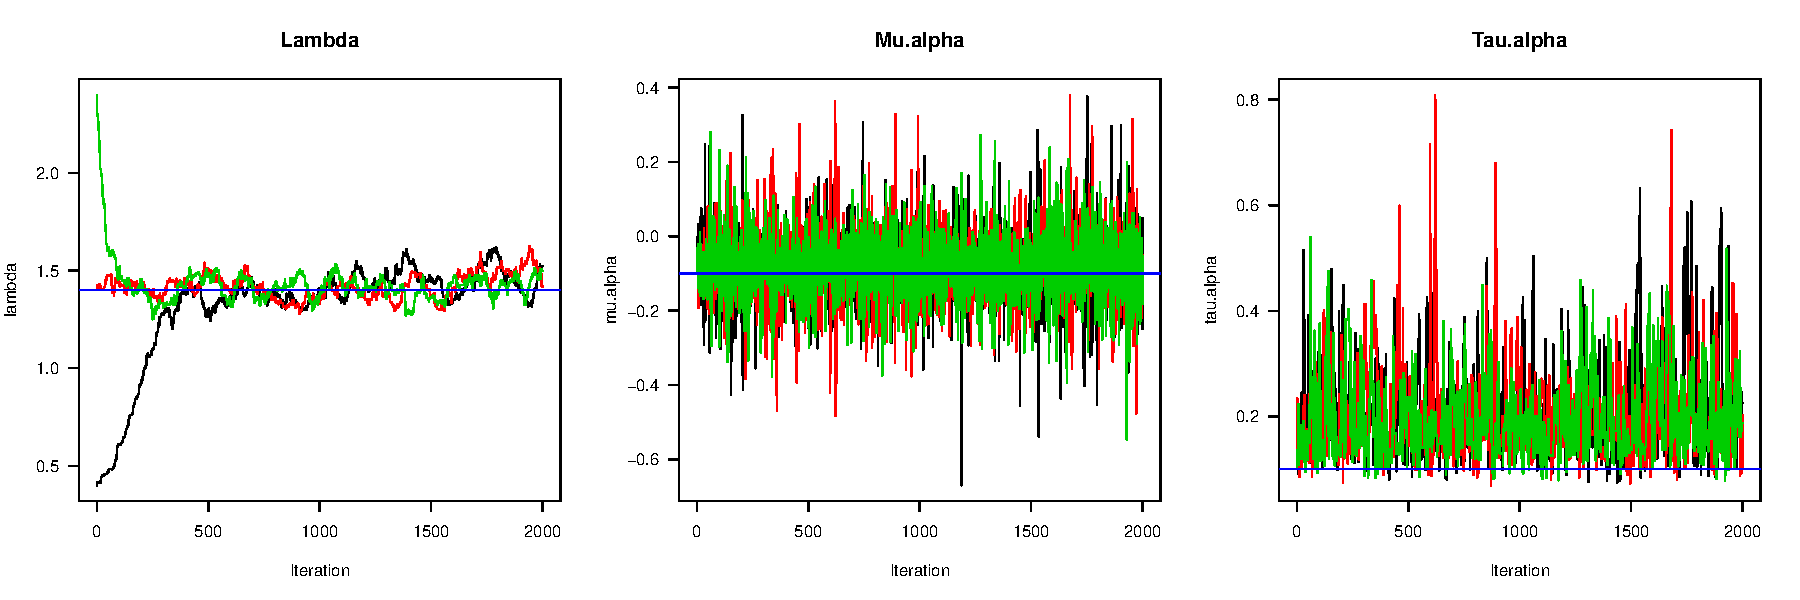
\includegraphics[width=6.0in]{fig_sim_sum1.pdf}
\caption{Simulation study results for $\lambda$, $\mu_\alpha$, and $\tau_\alpha$, where the horizontal blue lines represent the known true values of the parameters.}
\label{fig_sim_sum1}
\end{center}
\end{figure}


\section{Results}
The results on the real data are equally encouraging. 

1. prob and mean rainfall historical vs. sim\\

\begin{figure}[htbp]
\begin{center}
\includegraphics[width=6.0in]{Posterior_pwet_series1.pdf}
\includegraphics[width=6.0in]{Posterior_pwet_series3.pdf}
\includegraphics[width=6.0in]{Posterior_pwet_series4.pdf}
\includegraphics[width=6.0in]{Posterior_pwet_series8.pdf}
\includegraphics[width=6.0in]{Posterior_pwet_series9.pdf}
\caption{Simulation study results for $\lambda$, $\mu_\alpha$, and $\tau_\alpha$, where the horizontal blue lines represent the known true values of the parameters.}
\label{Posterior}
\end{center}
\end{figure}

2. dry spell historical vs sim

3. rainfall above a certain amount

3. metrics showing prob of rainfall in all locations?
onset and extremes


\section{Out-of Sample Predictions}

We also generate out of sample rainfall data using 2011's el nino data, and sampling from the posterior distribution from our initial run. We can compare these data to the actual weather time series for 2011 for: 


\end{document}




\hspace{0.3in} $Y_{stj} = 1(Z_{stj} > 0),$\\
\vspace{0.08in}
\hspace{0.3in} $Z_{stj} \sim N(W_{st} + \alpha_s X^\text{ARC}_{sj}, \tau_s^2),$\\
\vspace{0.08in}
\hspace{0.5in} $\bW_t \sim N_S(\bX_t \bbeta, \bR),$\\
\vspace{0.08in}
\hspace{0.7in} $\beta_{ps} \sim N(\mu_p, \sigma^2_p),$\\
\vspace{0.08in}
\hspace{0.7in} $\bR=\{r_{ik}\}$, $r_{ii}=1$, $r_{ik} = \exp(-\lambda d_{ik}), \hspace{1in} \text{for $i,k \in (1,..,S)$}$\\
\vspace{0.08in}
\hspace{0.7in} $\bX_t = (1,t,\sin(2\pi t \omega_1), \cos(2\pi t \omega_1),...),$\\
\vspace{0.08in}
\hspace{0.5in} $\alpha_s \sim N(\mu_\alpha, \tau^2_\alpha),$\\
\vspace{0.08in}
where we use relatively flat priors for $\tau$, $\mu_p$, $\sigma_p$, $\lambda$, $\mu_\alpha$, and $\tau_\alpha$.


